\documentclass[twoside]{book}

% Packages required by doxygen
\usepackage{fixltx2e}
\usepackage{calc}
\usepackage{doxygen}
\usepackage[export]{adjustbox} % also loads graphicx
\usepackage{graphicx}
\usepackage[utf8]{inputenc}
\usepackage{makeidx}
\usepackage{multicol}
\usepackage{multirow}
\PassOptionsToPackage{warn}{textcomp}
\usepackage{textcomp}
\usepackage[nointegrals]{wasysym}
\usepackage[table]{xcolor}

% Font selection
\usepackage[T1]{fontenc}
\usepackage[scaled=.90]{helvet}
\usepackage{courier}
\usepackage{amssymb}
\usepackage{sectsty}
\renewcommand{\familydefault}{\sfdefault}
\allsectionsfont{%
  \fontseries{bc}\selectfont%
  \color{darkgray}%
}
\renewcommand{\DoxyLabelFont}{%
  \fontseries{bc}\selectfont%
  \color{darkgray}%
}
\newcommand{\+}{\discretionary{\mbox{\scriptsize$\hookleftarrow$}}{}{}}

% Page & text layout
\usepackage{geometry}
\geometry{%
  a4paper,%
  top=2.5cm,%
  bottom=2.5cm,%
  left=2.5cm,%
  right=2.5cm%
}
\tolerance=750
\hfuzz=15pt
\hbadness=750
\setlength{\emergencystretch}{15pt}
\setlength{\parindent}{0cm}
\setlength{\parskip}{0.2cm}
\makeatletter
\renewcommand{\paragraph}{%
  \@startsection{paragraph}{4}{0ex}{-1.0ex}{1.0ex}{%
    \normalfont\normalsize\bfseries\SS@parafont%
  }%
}
\renewcommand{\subparagraph}{%
  \@startsection{subparagraph}{5}{0ex}{-1.0ex}{1.0ex}{%
    \normalfont\normalsize\bfseries\SS@subparafont%
  }%
}
\makeatother

% Headers & footers
\usepackage{fancyhdr}
\pagestyle{fancyplain}
\fancyhead[LE]{\fancyplain{}{\bfseries\thepage}}
\fancyhead[CE]{\fancyplain{}{}}
\fancyhead[RE]{\fancyplain{}{\bfseries\leftmark}}
\fancyhead[LO]{\fancyplain{}{\bfseries\rightmark}}
\fancyhead[CO]{\fancyplain{}{}}
\fancyhead[RO]{\fancyplain{}{\bfseries\thepage}}
\fancyfoot[LE]{\fancyplain{}{}}
\fancyfoot[CE]{\fancyplain{}{}}
\fancyfoot[RE]{\fancyplain{}{\bfseries\scriptsize Generated on Sun Jan 10 2016 16\+:51\+:45 for My Project by Doxygen }}
\fancyfoot[LO]{\fancyplain{}{\bfseries\scriptsize Generated on Sun Jan 10 2016 16\+:51\+:45 for My Project by Doxygen }}
\fancyfoot[CO]{\fancyplain{}{}}
\fancyfoot[RO]{\fancyplain{}{}}
\renewcommand{\footrulewidth}{0.4pt}
\renewcommand{\chaptermark}[1]{%
  \markboth{#1}{}%
}
\renewcommand{\sectionmark}[1]{%
  \markright{\thesection\ #1}%
}

% Indices & bibliography
\usepackage{natbib}
\usepackage[titles]{tocloft}
\setcounter{tocdepth}{3}
\setcounter{secnumdepth}{5}
\makeindex

% Hyperlinks (required, but should be loaded last)
\usepackage{ifpdf}
\ifpdf
  \usepackage[pdftex,pagebackref=true]{hyperref}
\else
  \usepackage[ps2pdf,pagebackref=true]{hyperref}
\fi
\hypersetup{%
  colorlinks=true,%
  linkcolor=blue,%
  citecolor=blue,%
  unicode%
}

% Custom commands
\newcommand{\clearemptydoublepage}{%
  \newpage{\pagestyle{empty}\cleardoublepage}%
}


%===== C O N T E N T S =====

\begin{document}

% Titlepage & ToC
\hypersetup{pageanchor=false,
             bookmarks=true,
             bookmarksnumbered=true,
             pdfencoding=unicode
            }
\pagenumbering{roman}
\begin{titlepage}
\vspace*{7cm}
\begin{center}%
{\Large My Project }\\
\vspace*{1cm}
{\large Generated by Doxygen 1.8.9.1}\\
\vspace*{0.5cm}
{\small Sun Jan 10 2016 16:51:45}\\
\end{center}
\end{titlepage}
\clearemptydoublepage
\tableofcontents
\clearemptydoublepage
\pagenumbering{arabic}
\hypersetup{pageanchor=true}

%--- Begin generated contents ---
\chapter{Cute\+Bode}
\label{md_README}
\hypertarget{md_README}{}
Cute\+Bode is a simple simulation software generating bode plots. 
\chapter{Hierarchical Index}
\section{Class Hierarchy}
This inheritance list is sorted roughly, but not completely, alphabetically\+:\begin{DoxyCompactList}
\item Q\+Graphics\+View\begin{DoxyCompactList}
\item \contentsline{section}{Plot}{\pageref{classPlot}}{}
\end{DoxyCompactList}
\item Q\+Main\+Window\begin{DoxyCompactList}
\item \contentsline{section}{Main\+Window}{\pageref{classMainWindow}}{}
\end{DoxyCompactList}
\item Q\+Object\begin{DoxyCompactList}
\item \contentsline{section}{Trf}{\pageref{classTrf}}{}
\end{DoxyCompactList}
\end{DoxyCompactList}

\chapter{Class Index}
\section{Class List}
Here are the classes, structs, unions and interfaces with brief descriptions\+:\begin{DoxyCompactList}
\item\contentsline{section}{\hyperlink{classMainWindow}{Main\+Window} }{\pageref{classMainWindow}}{}
\item\contentsline{section}{\hyperlink{classPlot}{Plot} }{\pageref{classPlot}}{}
\item\contentsline{section}{\hyperlink{classTrf}{Trf} }{\pageref{classTrf}}{}
\end{DoxyCompactList}

\chapter{Class Documentation}
\hypertarget{classMainWindow}{}\section{Main\+Window Class Reference}
\label{classMainWindow}\index{Main\+Window@{Main\+Window}}


Inheritance diagram for Main\+Window\+:

\hypertarget{classPlot}{}\section{Plot Class Reference}
\label{classPlot}\index{Plot@{Plot}}


Inheritance diagram for Plot\+:
\nopagebreak
\begin{figure}[H]
\begin{center}
\leavevmode
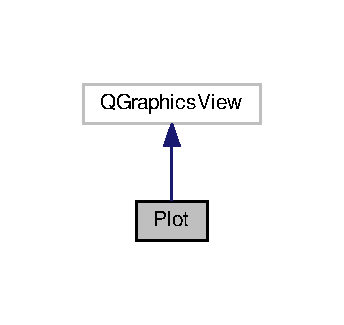
\includegraphics[width=165pt]{classPlot__inherit__graph}
\end{center}
\end{figure}


Collaboration diagram for Plot\+:
\nopagebreak
\begin{figure}[H]
\begin{center}
\leavevmode
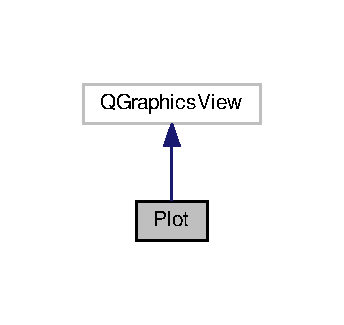
\includegraphics[width=165pt]{classPlot__coll__graph}
\end{center}
\end{figure}
\subsection*{Public Member Functions}
\begin{DoxyCompactItemize}
\item 
\hyperlink{classPlot_acb95c0d3a6d1d4edf7b946863efdac98}{Plot} (Q\+Widget $\ast$parent=0)
\begin{DoxyCompactList}\small\item\em \hyperlink{classPlot_acb95c0d3a6d1d4edf7b946863efdac98}{Plot\+::\+Plot}. \end{DoxyCompactList}\item 
void \hyperlink{classPlot_a1c6fda8fe644da0e0f0df6bf659455de}{calculate\+Magnitude} (Q\+List$<$ \hyperlink{classTrf}{Trf} $\ast$ $>$ trf\+List)
\begin{DoxyCompactList}\small\item\em \hyperlink{classPlot_a1c6fda8fe644da0e0f0df6bf659455de}{Plot\+::calculate\+Magnitude}. \end{DoxyCompactList}\item 
void \hyperlink{classPlot_afaf47513d7e2390b1c51df94a43a025e}{calculate\+Phase} (Q\+List$<$ \hyperlink{classTrf}{Trf} $\ast$ $>$ trf\+List)
\begin{DoxyCompactList}\small\item\em \hyperlink{classPlot_afaf47513d7e2390b1c51df94a43a025e}{Plot\+::calculate\+Phase}. \end{DoxyCompactList}\item 
void \hyperlink{classPlot_a8fae6078f872f751aa80d1f037266438}{plot} ()
\begin{DoxyCompactList}\small\item\em \hyperlink{classPlot_a8fae6078f872f751aa80d1f037266438}{Plot\+::plot}. \end{DoxyCompactList}\end{DoxyCompactItemize}
\subsection*{Public Attributes}
\begin{DoxyCompactItemize}
\item 
\hypertarget{classPlot_a25d9ba7cbbbb6af4be2fb5c51eb215fc}{}Q\+Vector$<$ Q\+Point\+F $\ast$ $>$ {\bfseries magnitude\+Points}\label{classPlot_a25d9ba7cbbbb6af4be2fb5c51eb215fc}

\item 
\hypertarget{classPlot_a7e4bee81b3be186f4ab225f75214c11b}{}Q\+Vector$<$ Q\+Point\+F $\ast$ $>$ {\bfseries phase\+Points}\label{classPlot_a7e4bee81b3be186f4ab225f75214c11b}

\item 
\hypertarget{classPlot_afdafdfe7409511731d871b9353f815e4}{}Q\+Vector$<$ Q\+Point\+F $\ast$ $>$ {\bfseries x\+Axis\+Points}\label{classPlot_afdafdfe7409511731d871b9353f815e4}

\end{DoxyCompactItemize}


\subsection{Constructor \& Destructor Documentation}
\hypertarget{classPlot_acb95c0d3a6d1d4edf7b946863efdac98}{}\index{Plot@{Plot}!Plot@{Plot}}
\index{Plot@{Plot}!Plot@{Plot}}
\subsubsection[{Plot}]{\setlength{\rightskip}{0pt plus 5cm}Plot\+::\+Plot (
\begin{DoxyParamCaption}
\item[{Q\+Widget $\ast$}]{parent = {\ttfamily 0}}
\end{DoxyParamCaption}
)\hspace{0.3cm}{\ttfamily [explicit]}}\label{classPlot_acb95c0d3a6d1d4edf7b946863efdac98}


\hyperlink{classPlot_acb95c0d3a6d1d4edf7b946863efdac98}{Plot\+::\+Plot}. 


\begin{DoxyParams}{Parameters}
{\em parent} & Konstruktor \\
\hline
\end{DoxyParams}


\subsection{Member Function Documentation}
\hypertarget{classPlot_a1c6fda8fe644da0e0f0df6bf659455de}{}\index{Plot@{Plot}!calculate\+Magnitude@{calculate\+Magnitude}}
\index{calculate\+Magnitude@{calculate\+Magnitude}!Plot@{Plot}}
\subsubsection[{calculate\+Magnitude}]{\setlength{\rightskip}{0pt plus 5cm}void Plot\+::calculate\+Magnitude (
\begin{DoxyParamCaption}
\item[{Q\+List$<$ {\bf Trf} $\ast$ $>$}]{trf\+List}
\end{DoxyParamCaption}
)}\label{classPlot_a1c6fda8fe644da0e0f0df6bf659455de}


\hyperlink{classPlot_a1c6fda8fe644da0e0f0df6bf659455de}{Plot\+::calculate\+Magnitude}. 


\begin{DoxyParams}{Parameters}
{\em trf\+List} & Berechnet den Betragsfrequenzgang \\
\hline
\end{DoxyParams}
\hypertarget{classPlot_afaf47513d7e2390b1c51df94a43a025e}{}\index{Plot@{Plot}!calculate\+Phase@{calculate\+Phase}}
\index{calculate\+Phase@{calculate\+Phase}!Plot@{Plot}}
\subsubsection[{calculate\+Phase}]{\setlength{\rightskip}{0pt plus 5cm}void Plot\+::calculate\+Phase (
\begin{DoxyParamCaption}
\item[{Q\+List$<$ {\bf Trf} $\ast$ $>$}]{trf\+List}
\end{DoxyParamCaption}
)}\label{classPlot_afaf47513d7e2390b1c51df94a43a025e}


\hyperlink{classPlot_afaf47513d7e2390b1c51df94a43a025e}{Plot\+::calculate\+Phase}. 


\begin{DoxyParams}{Parameters}
{\em trf\+List} & Berechnet den Phasenfrequenzgang \\
\hline
\end{DoxyParams}
\hypertarget{classPlot_a8fae6078f872f751aa80d1f037266438}{}\index{Plot@{Plot}!plot@{plot}}
\index{plot@{plot}!Plot@{Plot}}
\subsubsection[{plot}]{\setlength{\rightskip}{0pt plus 5cm}void Plot\+::plot (
\begin{DoxyParamCaption}
{}
\end{DoxyParamCaption}
)}\label{classPlot_a8fae6078f872f751aa80d1f037266438}


\hyperlink{classPlot_a8fae6078f872f751aa80d1f037266438}{Plot\+::plot}. 


\begin{DoxyItemize}
\item Löscht alten \hyperlink{classPlot}{Plot}
\item Erstellt Achsenkreuz
\item Malt die Funktion
\item Fügt Beschriftung der Achsen hinzu 
\end{DoxyItemize}

The documentation for this class was generated from the following files\+:\begin{DoxyCompactItemize}
\item 
plot.\+h\item 
plot.\+cpp\end{DoxyCompactItemize}

\hypertarget{classTrf}{}\section{Trf Class Reference}
\label{classTrf}\index{Trf@{Trf}}


Inheritance diagram for Trf\+:
\nopagebreak
\begin{figure}[H]
\begin{center}
\leavevmode
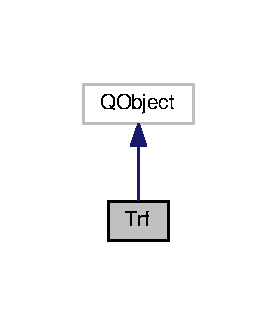
\includegraphics[width=133pt]{classTrf__inherit__graph}
\end{center}
\end{figure}


Collaboration diagram for Trf\+:
\nopagebreak
\begin{figure}[H]
\begin{center}
\leavevmode
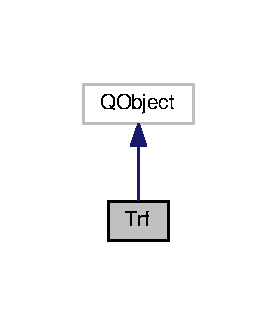
\includegraphics[width=133pt]{classTrf__coll__graph}
\end{center}
\end{figure}
\subsection*{Public Types}
\begin{DoxyCompactItemize}
\item 
\hypertarget{classTrf_a95d5a31d33597372b88527b4072246fb}{}enum {\bfseries Type} \{ {\bfseries Type1}, 
{\bfseries Type2}, 
{\bfseries Type3}, 
{\bfseries Type4}
 \}\label{classTrf_a95d5a31d33597372b88527b4072246fb}

\end{DoxyCompactItemize}
\subsection*{Public Member Functions}
\begin{DoxyCompactItemize}
\item 
\hyperlink{classTrf_a7e7c53f1e2e7f15e416bcffc6d259425}{Trf} (Q\+Object $\ast$parent=0)
\begin{DoxyCompactList}\small\item\em \hyperlink{classTrf_a7e7c53f1e2e7f15e416bcffc6d259425}{Trf\+::\+Trf}. \end{DoxyCompactList}\item 
Trf\+::\+Type \hyperlink{classTrf_a83cfd9d1f9feb5666f9222041d9d8c71}{get\+Type} ()
\begin{DoxyCompactList}\small\item\em \hyperlink{classTrf_a83cfd9d1f9feb5666f9222041d9d8c71}{Trf\+::get\+Type}. \end{DoxyCompactList}\item 
void \hyperlink{classTrf_a3fe2a559037af5cfaa9a07d1f34601c4}{set\+Type} (Type t)
\begin{DoxyCompactList}\small\item\em \hyperlink{classTrf_a3fe2a559037af5cfaa9a07d1f34601c4}{Trf\+::set\+Type}. \end{DoxyCompactList}\item 
double \hyperlink{classTrf_a6e366454617b79c90927624f025f222f}{get\+Tau} ()
\begin{DoxyCompactList}\small\item\em \hyperlink{classTrf_a6e366454617b79c90927624f025f222f}{Trf\+::get\+Tau}. \end{DoxyCompactList}\item 
void \hyperlink{classTrf_a4162a49bf984baaf406409ab3cd8f029}{set\+Tau} (double t)
\begin{DoxyCompactList}\small\item\em \hyperlink{classTrf_a4162a49bf984baaf406409ab3cd8f029}{Trf\+::set\+Tau}. \end{DoxyCompactList}\end{DoxyCompactItemize}


\subsection{Constructor \& Destructor Documentation}
\hypertarget{classTrf_a7e7c53f1e2e7f15e416bcffc6d259425}{}\index{Trf@{Trf}!Trf@{Trf}}
\index{Trf@{Trf}!Trf@{Trf}}
\subsubsection[{Trf}]{\setlength{\rightskip}{0pt plus 5cm}Trf\+::\+Trf (
\begin{DoxyParamCaption}
\item[{Q\+Object $\ast$}]{parent = {\ttfamily 0}}
\end{DoxyParamCaption}
)\hspace{0.3cm}{\ttfamily [explicit]}}\label{classTrf_a7e7c53f1e2e7f15e416bcffc6d259425}


\hyperlink{classTrf_a7e7c53f1e2e7f15e416bcffc6d259425}{Trf\+::\+Trf}. 


\begin{DoxyParams}{Parameters}
{\em parent} & Konstruktor der Transferfunktion \\
\hline
\end{DoxyParams}


\subsection{Member Function Documentation}
\hypertarget{classTrf_a6e366454617b79c90927624f025f222f}{}\index{Trf@{Trf}!get\+Tau@{get\+Tau}}
\index{get\+Tau@{get\+Tau}!Trf@{Trf}}
\subsubsection[{get\+Tau}]{\setlength{\rightskip}{0pt plus 5cm}double Trf\+::get\+Tau (
\begin{DoxyParamCaption}
{}
\end{DoxyParamCaption}
)}\label{classTrf_a6e366454617b79c90927624f025f222f}


\hyperlink{classTrf_a6e366454617b79c90927624f025f222f}{Trf\+::get\+Tau}. 

\begin{DoxyReturn}{Returns}
Tau Gibt den Wert Tau der Teilfunktion zurück 
\end{DoxyReturn}
\hypertarget{classTrf_a83cfd9d1f9feb5666f9222041d9d8c71}{}\index{Trf@{Trf}!get\+Type@{get\+Type}}
\index{get\+Type@{get\+Type}!Trf@{Trf}}
\subsubsection[{get\+Type}]{\setlength{\rightskip}{0pt plus 5cm}Trf\+::\+Type Trf\+::get\+Type (
\begin{DoxyParamCaption}
{}
\end{DoxyParamCaption}
)}\label{classTrf_a83cfd9d1f9feb5666f9222041d9d8c71}


\hyperlink{classTrf_a83cfd9d1f9feb5666f9222041d9d8c71}{Trf\+::get\+Type}. 

\begin{DoxyReturn}{Returns}
type Gibt den Typ der Teilfunktion zurück 
\end{DoxyReturn}
\hypertarget{classTrf_a4162a49bf984baaf406409ab3cd8f029}{}\index{Trf@{Trf}!set\+Tau@{set\+Tau}}
\index{set\+Tau@{set\+Tau}!Trf@{Trf}}
\subsubsection[{set\+Tau}]{\setlength{\rightskip}{0pt plus 5cm}void Trf\+::set\+Tau (
\begin{DoxyParamCaption}
\item[{double}]{t}
\end{DoxyParamCaption}
)}\label{classTrf_a4162a49bf984baaf406409ab3cd8f029}


\hyperlink{classTrf_a4162a49bf984baaf406409ab3cd8f029}{Trf\+::set\+Tau}. 


\begin{DoxyParams}{Parameters}
{\em t} & Setzt den Wert Tau der Teilfunktion \\
\hline
\end{DoxyParams}
\hypertarget{classTrf_a3fe2a559037af5cfaa9a07d1f34601c4}{}\index{Trf@{Trf}!set\+Type@{set\+Type}}
\index{set\+Type@{set\+Type}!Trf@{Trf}}
\subsubsection[{set\+Type}]{\setlength{\rightskip}{0pt plus 5cm}void Trf\+::set\+Type (
\begin{DoxyParamCaption}
\item[{Type}]{t}
\end{DoxyParamCaption}
)}\label{classTrf_a3fe2a559037af5cfaa9a07d1f34601c4}


\hyperlink{classTrf_a3fe2a559037af5cfaa9a07d1f34601c4}{Trf\+::set\+Type}. 


\begin{DoxyParams}{Parameters}
{\em t} & Setz den Typ der Teilfunktion \\
\hline
\end{DoxyParams}


The documentation for this class was generated from the following files\+:\begin{DoxyCompactItemize}
\item 
trf.\+h\item 
trf.\+cpp\end{DoxyCompactItemize}

%--- End generated contents ---

% Index
\backmatter
\newpage
\phantomsection
\clearemptydoublepage
\addcontentsline{toc}{chapter}{Index}
\printindex

\end{document}
